% Chapter Template

\chapter{Diseño e Implementación} % Main chapter title
% cSpell:words resizebox onosapi usecase Mcast enrutamiento parencite includegraphics pcktprocactiv lstlisting iperf

\label{Chapter4} % Change X to a consecutive number; for referencing this chapter elsewhere, use 
% \ref{ChapterX} 
Para el desarrollo del proyecto, será necesario implementar un sistema en donde se puedan realizar pruebas y evaluar de este modo la correctitud del mismo. 

De esta forma, la primera sección de este capítulo comprende tanto el análisis del sistema como la topología utilizada. Específicamente, se estudiará su estructura, su comportamiento y sus requerimientos. 

En las secciones siguientes, se detallan las diferentes aplicaciones desarrolladas que permiten cumplir con el objetivo del proyecto. En primer lugar, se hará un estudio del módulo YANG implementado, el cual caracteriza y modela los datos del equipo. A continuación, se detallará el driver implementado para lograr la comunicación entre el controlador y el dispositivo. Por último, se analizará la interfaz REST y la GUI desarrollada.

%----------------------------------------------------------------------------------------
%	SECTION 1
%----------------------------------------------------------------------------------------

\section{Entorno de trabajo}
En esta sección se detallan las características del sistema a implementar, descriptas en el lenguaje de especificación de sistemas SysML \parencite{sysml}. Se optó por este lenguaje de modelado ya que brinda una extensión a UML permitiendo combinar elementos del mundo físico (\textit{hardware}) con elementos del mundo lógico (\textit{software}). 

%-----------------------------------
%	SUBSECTION 1
%-----------------------------------

\subsection{Topología}

Con el fin de poder identificar en una primera instancia los requerimientos que debe cumplir el sistema, se conformará una topología. La misma, está basado en un caso de uso simple en el cual se quiere brindar conectividad a dos clientes a través de un enlace óptico, este último conformado por dos \textit{muxponders}.  

Además, es importante identificar la presencia del controlador, el cual gestionará la configuración de los equipos mediante el protocolo \textit{NETCONF}. En la figura \ref{fig:topologia} se muestra de forma general la topología planteada.

\begin{figure}[H]
    \centering
    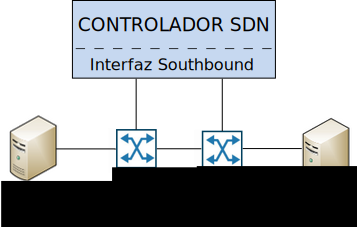
\includegraphics[scale=0.85]{Figures/topologia.pdf}
    \caption{Topología implementada en el proyecto.}
    \label{fig:topologia}
  \end{figure}


Los dispositivos terminales A y B, se encuentran conectados cada uno a los puertos cliente del \textit{muxponder} de 40Gb. A su vez, el transmisor del \textit{muxponder} C se encuentra conectado con el receptor del \textit{muxponder} D, y viceversa. Esto permite una comunicación bidireccional, donde ambos clientes pueden tener conectividad. 

A continuación, en la figura \ref{fig:topologiafis} se muestra como está dispuesta la conexión físicamente en los dispositivos. A la izquierda se tiene el \textit{muxponder} C, y a la derecha se encuentra el \textit{muxponder} D. Las interfaces de control de ambos dispositivos están conectadas al controlador \textit{ONOS}, mientras que los puertos clientes se encuentran conectados a los clientes A y B respectivamente. Por otra parte, las interfaces de línea se encuentran conectados entre los \textit{muxponder}, como se explicó anteriormente, con el fin de poder tener una comunicación bidireccional.

\begin{figure}[H]
    \centering
    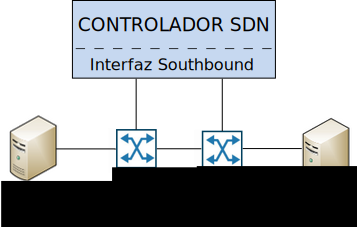
\includegraphics[scale=0.7]{Figures/topologia.pdf}
    \caption{Conexión física de la topología.}
    \label{fig:topologiafis}
  \end{figure}

\subsection{Requerimientos del sistema}

Para establecer los requerimientos funcionales del sistema, se presentará en primera instancia, diagramas de casos de usos. Como se puede observar en el diagrama de la figura \ref{fig:caso_uso_admin}, el objeto principal del sistema es poder brindar al administrador un entorno donde el mismo pueda gestionar a los muxponders mediante sus aplicaciones.

\begin{figure}[H]
    \centering
    \includegraphics[scale=0.55]{Figures/caso_uso_admin.pdf}
    \caption{Caso de uso desde la perspectiva del administrador.}
    \label{fig:caso_uso_admin}
  \end{figure}

  En base a esto, se pueden definir los requerimientos funcionales a nivel de sistema. La figura \ref{fig:req_sys} muestra una lista de los mismos. 
  
  Como requerimiento no funcional, se puede identificar la adición de nodos virtuales, los cuales no afectan a la funcionalidad del sistema pero brindan más flexibilidad y permiten conformar una topología más compleja. Dichos nodos consistirán en switches virtuales conectados a los muxponders, y a su vez conectados con host virtuales.

  \begin{figure}[H]
    \centering
    \includegraphics[scale=0.65]{Figures/req_sys.pdf}
    \caption{Requerimientos del sistema.}
    \label{fig:req_sys}
  \end{figure}


  Además, a partir del diagrama de caso de uso de la figura \ref{fig:caso_uso_admin}, se pueden identificar tres diagramas de actividades relacionadas. 
  \\

  En la figura \ref{fig:actividad_config}, se observa el flujo de actividad típico que tendrá una operación de configuración por parte del administrador. Como se puede ver, el evento inicial es la adición de una configuración desde la aplicación web. Esta configuración, una vez procesada, se traduce en una solicitud POST HTTP que se envían hacia la northbound interface del controlador. Una vez recibida la solicitud, se realiza su procesamiento y se envía el mensaje de configuración NETCONF a los dispositivos involucrados a través de la southbound interface.

  Por otra parte, la actividad de monitoreo se observa en la figura \ref{fig:actividad_config}, donde la aplicación realiza consultas periódicas al controlador para obtener información sobre los dispositivos. Se envía un mensaje HTTP, (esta vez una operación GET), el controlador procesa la petición para responder nuevamente la consulta.

  Por último, en la figura \ref{fig:actividad_config} se tiene el flujo de actividades donde el controlador registra una alarma mediante una notificación NETCONF que envía un dispositivo.


  \begin{figure}[H]
    \centering
    \includegraphics[scale=0.40]{Figures/actividad_config.pdf}
    \caption{Topología implementada en el proyecto.}
    \label{fig:actividad_config}
  \end{figure}


  \section{Integración del protocolo NETCONF al muxponder}
  La sección anterior, deja claro que uno de los requerimientos de sistema será que tanto el controlador ONOS como los dispositivos a monitorear, soporten NETCONF como protocolo de gestión de la configuración. 
  
  Como se vio en el capítulo anterior, el controlador soporta dicho protocolo, por lo que para cumplir con este requisito de sistema, únicamente será necesario adaptar NETCONF al dispositivo. 
  
  \subsection{Requerimientos para la integración del protocolo}

  Para cumplir con los requerimientos vistos en \ref{fig:req_sys}, se confeccionaron los requerimientos que se observan en la figura [X].

  \begin{figure}[H]
    \centering
    \includegraphics[scale=0.65]{Figures/req_sys.pdf}
    \caption{Topología implementada en el proyecto.}
    \label{fig:req_sys}
  \end{figure}

  \subsection{Compilación instalación del agente}
Siendo YUMA123 el agente que se eligió para integrar el protocolo NETCONF en el equipo, en esta sección se detalla el procedimiento que se llevó a cabo para la compilación e instalación del agente en el muxponder, con el fin de poder cumplir el requerimiento R-07.
\\

  En primer lugar, toda la tarea de compilación se realizó en una computadora de propósito general, debido a los recursos limitados con los que cuenta el dispositivo. Para facilitar la compilación e instalación, se realizaron tres scripts los cuales se describen a continuación:

  \begin{itemize}
	\item \textbf{Dockerfile}: el objetivo de este script, es el de realizar la compilación del proyecto YUMA123, dejando todas las librerías y los binarios en una carpeta que luego deberá copiarse en el dispositivo. Dockerfile [] es un archivo de texto que contiene los pasos e instrucciones que la herramienta Docker deberá seguir para construir una imagen. En el mismo, se indica una imagen de referencia (ubuntu:16.04) que servirá como base para la construcción. Luego, se descargan todas las librerías requeridas por el proyecto YUMA123 junto con los compiladores necesarios para realizar la compilación cruzada. A partir de aquí, se compila cada una de las librerías para la arquitectura objetivo (por ejemplo, NIOS II) y finalmente se compila también el proyecto YUMA123. Todos los binarios, librerías y cabeceras resultantes se encuentran en la carpeta “$/root/usrapp$” de la imagen Docker construida. Cabe destacar que de esta forma se realizaron tres versiones del script, con el objetivo de poder compilar para las arquitecturas NIOS II, ARM y 86 64.
    
    \item \textbf{$remote_install_yuma.sh$}: script bash que tiene la tarea de realizar la instalación del protocolo compilado previamente con Docker y Dockerfile. Para ello, requiere de tres parámetros: usuario del dispositivo remoto, dirección IP del dispositivo remoto y la arquitectura deseada. Con estos parámetros, el script realiza la instalación del protocolo NETCONF mediante SSH y SCP [], copiando el contenido necesario de "$/root/usrapp$" que se generó con la construcción de la imagen Docker, al directorio "$/root/usrapp$" del dispositivo. Es importante mencionar que muchas de las librerías requeridas por YUMA123 son necesarias únicamente para la compilación y no para el funcionamiento del protocolo, por lo que este script omitirá dichas librerías con el fin de reducir el tamaño que ocupa el agente en memoria.
    
    \item \textbf{$remote_uninstall_yuma.sh$}: requiere dos parametros los cuales son el usuario del dispositivo remoto y la dirección ip del mismo. El objetivo de este script es facilitar la desinstalación de todas las librerías relacionadas a YUMA123 del dispositivo.

\end{itemize}


\subsection{Diseño del módulo YANG}

Para poder cumplir con los requerimientos R-08, R-09 y R-10 que se muestra en la figura [X], se diseñó un módulo YANG que contiene cinco secciones bien definidas, las cuales se describen a continuación: 

\begin{itemize}
	\item \textbf{Cabecera del módulo y declaraciones}: contiene la estructura inicial de un módulo YANG. En él, se define un nombre y un prefijo, se realiza una descripción del mismo y por último se realiza la definición de los datos utilizados por el módulo. Cabe destacar que se definieron tres tipos de datos: restricted-tipo-trafico, restricted-tipo-fec-linea y restricted-tipo-fec-cliente, donde se especifica a través de la directiva ‘enum’, cuales son los valores aceptados que puede tomar dicho tipo de dato. Por ejemplo, dado que la configuración del tipo de tráfico para este dispositivo únicamente admite dos valores (otu2 y xge), es importante restringir el ingreso de algún otro valor ya que podría ocasionar errores en la configuración. Se puede observar un fragmento del módulo realizado en la figura [X], donde se detalla la cabecera del módulo y sus declaraciones.  

    \begin{lstlisting}[language=SHELXL, caption=Interacción tipica con un dispositivo mediante \textit{CLI}., label=lstlisting:cli]
        module cli-mxp {

            namespace "http://fulgor.com/ns/cli-mxp";
            prefix "cli-mxp";
        
            description
              "CLI para configurar el muxponder de 40G";
        
            revision "2018-06-24" {
                description
                  "Version 0.1.0";
            }
            
            typedef restricted-tipo-trafico {
                type enumeration {
                    enum "otu2";
                    enum "xge";
                  }
            }
        
              ...
              ...
              ...
    \end{lstlisting}

    \item \textbf{Container YANG de configuración}: el módulo contiene también una sección donde se declara un container llamado ‘mux-config’, el cual es el único que admite datos de configuración del dispositivo. En él, se describen todos los parámetros que admiten una configuración (por ejemplo, el tipo de fec de línea), a través de las declaraciones ‘leaf’. Un fragmento de esta sección puede observarse en la figura [X], donde además se ve el uso de los tipos de datos definidos en la cabecera del módulo.
  
    \begin{lstlisting}[language=SHELXL, caption=Interacción tipica con un dispositivo mediante \textit{CLI}., label=lstlisting:cli]
    container mux-config {
        description "Parametros de la CLI";

        leaf tipo_trafico {
            description
              "[otu2|xge] especifica el tipo de tráfico.";
            type restricted-tipo-trafico;
        }
      
      ...
      ...
      ...
        
        list ports {
            key "port";
            leaf port {
                type int16{
                    range "0 .. 6";
                }
                mandatory true;
            }

            leaf neighbor {
                mandatory true;
                type string;
            }
            
            leaf port_neighbor {
                mandatory true;
                type string;
            }
        }
    }
    \end{lstlisting}

    \item \textbf{Container YANG de estado}: de igual forma, se realizaron containers para los datos de estado, los cuales no admiten una escritura de valores y son necesarios para monitoreo del dispositivo. La figura [X] muestra una parte de esta sección del módulo, donde puede apreciarse la directiva “config false”, la cual indica que el container no admitirá datos de configuración.  

    \begin{lstlisting}[language=SHELXL, caption=Interacción tipica con un dispositivo mediante \textit{CLI}., label=lstlisting:cli]
    container mux-state {
        description "Representa a datos de estado del dispositivo.";
        
        config false;

        leaf fpga_temperature_state {
            description "Temperatura de la FPGA";
            type decimal64 {
                fraction-digits 2;
            }
        }
   
        leaf device_boardId {
            description "Identificador unico del dispositivo";
            type string;
        }
        ...
        ...
        ...
    \end{lstlisting}


    \item \textbf{Definición de RPC}: Como se estudió en capítulos anteriores, NETCONF permite definir RPC propias de un módulo, con el fin de extender la funcionalidad de los dispositivos. Se define así una RPC cuya utilidad será la de poder indicar al agente cuándo debe aplicar la configuración que contiene el container “mux-config” en el dispositivo. En la figura [X], se muestra dicha sección del módulo, en ella se puede notar que la RPC admite una respuesta de la operación solicitada, la cual está contenida en el leaf “respuesta-mux-apply-config” y es de tipo String. En este mensaje se indica el resultado de la operación.


    \begin{lstlisting}[language=SHELXL, caption=Interacción tipica con un dispositivo mediante \textit{CLI}., label=lstlisting:cli]
    rpc mux-apply-config {        
        description "RPC que aplica los cambios de configuracion";
        output {
            leaf respuesta-mux-apply-config {
                type string;
            }
        }
    }
    \end{lstlisting}

    \item \textbf{Definición de notificación}: por último, el módulo tiene una sección donde se declara una notificación. Dicho mensaje será utilizado para indicar a las sesiones conectadas y suscritas, las diferentes alarmas que produzca el dispositivo. Estos mensajes se transportan mediante notificaciones del protocolo NETCONF.  La idea de estos mensajes es la de, por ejemplo, poder notificar mediante una alarma si un enlace con un dispositivo vecino se cayó, si el dispositivo supera la temperatura umbral, etc. La figura [x] muestra la declaración de dicha notificación en el módulo, donde se puede ver que el mensaje estará contenido dentro de la leaf “INFO”, en la cual se especifica de forma obligatoria con la directiva “mandatory”, cuál será el mensaje que se enviará como notificación.


    \begin{lstlisting}[language=SHELXL, caption=Interacción tipica con un dispositivo mediante \textit{CLI}., label=lstlisting:cli]
    notification mux-notify {
        leaf INFO {
            type string;
            mandatory "true";
        }
    }
    \end{lstlisting}

\end{itemize}

\subsection{Diseño de la librería C para el agente NETCONF}
Para comprender el funcionamiento de la librería desarrollada, será importante mencionar dos binarios que incorporan los muxponders de 40Gb: monitor y ñññññññññ. 

Para permitir que otros procesos conozcan el estado del dispositivo, el equipo utiliza el método de comunicación entre procesos llamado memoria compartida. El mismo, consiste en una región de memoria donde se permite que otras aplicaciones puedan, por ejemplo, leer información. 

Así, la aplicación “monitor” es utilizado por el muxponder para actualizar en dicha zona de memoria, los valores de las diferentes variables del dispositivo. Además, el binario mencionado también tiene la tarea de mostrar en la CLI, la información de estas variables. 

La figura [x] muestra el binario monitor en ejecución.

\begin{figure}[H]
    \centering
    \includegraphics[scale=0.65]{Figures/req_sys.pdf}
    \caption{Topología implementada en el proyecto.}
    \label{fig:req_sys}
  \end{figure}

  Por otra parte, la aplicación ñññññññññ es utilizada por el administrador para poder configurar el dispositivo mediante ciertos parámetros que son especificados haciendo uso de la CLI del equipo. Por ejemplo, con esta aplicación, el administrador podría cambiar la configuración de un equipo que tiene un tipo de tráfico xge por un tipo de tráfico otu2 a través de la CLI. Se ejemplifica lo mencionado anteriormente en la figura [X].

  \begin{figure}[H]
    \centering
    \includegraphics[scale=0.65]{Figures/req_sys.pdf}
    \caption{Topología implementada en el proyecto.}
    \label{fig:req_sys}
  \end{figure}

  Teniendo en cuenta las aplicaciones mencionadas, se procede a explicar el diseño de la librería en el lenguaje C. Para ello, se utilizó la herramienta yangdump del proyecto YUMA123, la cual genera un esqueleto de la aplicación a partir de un módulo YANG dado. Se forman así dos archivos, uno con extensión .h (headers) y otro con extensión .c (código fuente). 
  \\

  En el primero, la herramienta declara todas las variables, funciones y los tipos de datos que va a utilizar la librería. Este archivo es incluido en el archivo con extensión .c mediante la directiva “include” en C.

  El segundo archivo contiene la estructura de la aplicación en sí. En ella, se encuentran implementadas todas las funciones, las cuales llamara el agente en caso de que ingrese un mensaje referido al módulo YANG en cuestión. Todo el desarrollo de la aplicación y la relación entre la instrumentación del dispositivo con el módulo YANG, se encuentra en este archivo. 
  \\

  Con el fin de explicar cómo se desarrolló esta aplicación, se distinguen dos flujos de actividades bien definidos, uno para las operaciones que son sincrónicas con los mensajes que envía el cliente, y otro para aquellas que sean asíncronas a los mensajes del mismo. 

  Para el primer grupo, se tiene entonces las operaciones como obtención de un dato de estado o de configuración, modificación de un dato de configuración y ejecución de RPC, mientras que el segundo grupo contempla el envío de notificaciones, las cuales son asíncronas a las operaciones del cliente.
  \\

  Se muestra el comportamiento del primer grupo en el diagrama de actividad de la figura [X]. Cada vez que llega un mensaje NETCONF al agente YUMA123, el mismo procesa y verifica a qué módulo YANG hace referencia el mensaje y qué tipo de operación requiere el cliente. 

  Si la operación es una consulta por una variable de estado o de configuración, el agente realiza una llamada a una función relacionada a la variable consultada. En dicha función, lo que se hace es tomar el valor de memoria compartida del dispositivo, castear el mismo según indique el modulo YANG (string, int, uint, etc) y por ultimo, emitir una respuesta al cliente con el valor del dato consultado.

  Por otra parte, si la operación es la de editar una variable de configuración, el agente llama a una función de la librería C relacionada al módulo en cuestión, donde se actualiza el valor de dicha variable. Además, el agente emite un mensaje con el resultado de la operación. 

  Por último, si la operación trata de una RPC definida en el módulo YANG, el agente llama a la función relacionada a la RPC para efectuar la tarea solicitada. En este caso, se tiene una RPC que indica cuándo se deberá aplicar la configuración en el dispositivo, por lo que al momento de llamar a esta RPC, el agente copia los valores de los datos de configuración necesarios (tipo de tráfico, tipo fec de cliente, tipo fec línea, etc) y los aplica haciendo uso del binario ñññññññ explicado anteriormente.

  \begin{figure}[H]
    \centering
    \includegraphics[scale=0.65]{Figures/req_sys.pdf}
    \caption{Topología implementada en el proyecto.}
    \label{fig:req_sys}
  \end{figure}

  Por otra parte, el grupo relacionado a las operaciones asíncronas con los mensajes del cliente, no es otra cosa que la operación de envío de notificaciones mediante el protocolo NETCONF. Para ello, la librería desarrollada en C, crea un hilo que examina periódicamente cada tres segundos la memoria compartida del dispositivo. 
  
  La razón por la cual se examina cada tres segundos, está relacionada con la aplicación “monitor”, la cual actualiza los valores de memoria compartida con esa frecuencia.

  Al examinar los valores de las alarmas, las compara con la información antigua que se tenía almacenada sobre las mismas. Si la información es igual, no se envían notificaciones a las sesiones. En cambio, si la información actual es diferente a la información anterior, quiere decir que existe un cambio de estado de la misma y por lo tanto será necesario notificar a las sesiones suscritas este nuevo estado de las alarmas. Así, tanto el nombre de la alarma como el nuevo estado, son enviados a través de la notificación definida en la figura [X], haciendo uso de la leaf INFO.
  
  Un diagrama de actividad de estas operaciones se puede observar en la figura [X].

  \begin{figure}[H]
    \centering
    \includegraphics[scale=0.65]{Figures/req_sys.pdf}
    \caption{Topología implementada en el proyecto.}
    \label{fig:req_sys}
  \end{figure}


  \section{Diseño del Driver}
  Como se vio en capítulos anteriores, ONOS se comunica con los dispositivos a través de tres componentes de la interfaz Southbound: Providers, Protocols y Drivers.
  
  Así, para poder indicar al controlador cuáles serán las operaciones y los comportamientos específicos del muxponder de 40Gb, será necesario desarrollar un Driver (Java) en la interfaz Southbound del controlador. 

  \subsection{Requerimientos del Driver}
  A fin de cubrir las necesidades del administrador, visto en el caso de uso de la figura X, el Driver desarrollado deberá cumplir con los requerimientos funcionales del a figura [X].
  
  \begin{figure}[H]
    \centering
    \includegraphics[scale=0.65]{Figures/req_sys.pdf}
    \caption{Topología implementada en el proyecto.}
    \label{fig:req_sys}
  \end{figure}

  \subsection{Descubrimiento del dispositivo}
  El controlador ONOS reconoce la presencia de un nuevo dispositivo a través de un mensaje en formato JSON, el cual contiene información como la dirección IP del equipo, el driver que describe sus comportamientos, el protocolo que utiliza, entre otra información de utilidad. 
  
  Un ejemplo de este mensaje se muestra en la figura [X]. Dicho mensaje, es enviado al controlador haciendo uso del comando de ONOS “onos-netcfg” [].

  \begin{lstlisting}[language=SHELXL, caption=Interacción tipica con un dispositivo mediante \textit{CLI}., label=lstlisting:cli]
    {
        "devices": {
            "netconf:172.16.0.141:830": {
            "netconf": {
                "ip": "172.16.0.141",
                "port": 830,
                "username": "user",
                "password": "pass",
            },
            "basic": {
                "driver": "altura-netconf"
           }
        }
    }
    \end{lstlisting}


    Al momento de indicar al controlador ONOS la presencia de un nuevo dispositivo, el mismo hace una llamada por única vez a la función DeviceDescriptionDiscovery, la cual se encuentra implementada en el Driver indicado por el archivo JSON. 

    Esta función, tiene la tarea de descubrir las características más generales del equipo, como ser la versión de software y de hardware del mismo, el número de puertos disponibles, el identificador único del dispositivo, etc.

    Con más detalle, lo que realiza la función es iniciar la sesión SSH del protocolo NETCONF, esperar a que termine el intercambio de capacidades entre cliente y servidor y por último, enviar un mensaje NETCONF al servidor solicitando con la operación “GET”, los siguientes datos de estado:  información del fabricante, versión del hardware, software, identificador único del equipo y las alarmas que estén activas. 

    Como se aclaró, en esta función también se debe realizar el descubrimiento de los puertos del dispositivo, pero como estos no cambian a lo largo de la vida del equipo, no se envía un mensaje al servidor solicitando información de los mismos, sino que la información se encuentra especificada en el propio Driver.

    La figura [x] muestra el flujo de actividad típico que tendría el controlador ONOS al momento de agregarse un nuevo dispositivo administrado por el Driver desarrollado.
    
    \begin{figure}[H]
        \centering
        \includegraphics[scale=0.65]{Figures/req_sys.pdf}
        \caption{Topología implementada en el proyecto.}
        \label{fig:req_sys}
      \end{figure}

\subsection{Descubrimiento de Enlaces}

El Driver también debe proveer un mecanismo para indicar al controlador cómo se componen los enlaces entre los diferentes dispositivos administrados. Para ello, el controlador ONOS brinda una interfaz llamada “LinkDiscovery”, la cual se deberá implementar en el driver desarrollado. 

Así, el controlador llama periódicamente a esta función (cada 30 segundos de forma predeterminada, pudiéndose cambiar este tiempo desde la CLI) para corroborar el estado de los enlaces. 

Con más detalle, lo que realiza esta función es enviar periódicamente a los dispositivos un mensaje NETCONF con la operación GET-CONFIG, consultando por los datos “port”, “neighbor” y “port-neighbor” del container mux-config, estos datos pueden verse representados en el módulo YANG, en la figura [X]. A continuación, se explica de forma breve la función de cada uno de estos datos:

\begin{itemize}
	\item \textbf{port}: indica el puerto del dispositivo local al cual se conectará un vecino.
    
    \item \textbf{neighbor}: contiene el identificador único del dispositivo vecino al que se hace referencia en “port”.
    
    \item \textbf{port}: indica el puerto del dispositivo vecino con el que se deberá formar el enlace.
\end{itemize}

Con esta información, el controlador comprueba si el dispositivo local o el vecino tienen alarmas registradas respecto al enlace de línea del muxponder, concretamente lo hace mediante las alarmas “RXS” y “Rx LOCK ERR”. 

Si alguno de los dispositivos involucrados contiene una de estas alarmas, el enlace no se forma. De lo contrario, si no tienen estas alarmas, el driver informa al controlador que forme un enlace óptico entre ambos dispositivos. El diagrama de actividad de la figura [X] muestra lo explicado anteriormente.

\begin{figure}[H]
    \centering
    \includegraphics[scale=0.65]{Figures/req_sys.pdf}
    \caption{Topología implementada en el proyecto.}
    \label{fig:req_sys}
  \end{figure}

  Es importante notar que en esta instancia, no se consulta al dispositivo por sus alarmas con un mensaje NETCONF, ya que las mismas son enviadas asíncronamente mediante notificaciones NETCONF por el dispositivo, y registradas por el controlador como alarmas. Por lo tanto, para verificar el estado de las alarmas de un dispositivo, solo se consulta internamente en el core de ONOS.

  \subsection{Operaciones definidas en el Driver}

  El driver desarrollado brinda, además de las implementaciones de LinkDiscovery y DeviceDescriptionDiscovery explicadas anteriormente, interfaces a todas las operaciones admitidas por el dispositivo, entre ellas la RPC que se describió en la figura [X]. Esto es necesario para que luego, las diferentes aplicaciones de la capa de aplicación, puedan comunicarse con el dispositivo a través del driver. 

  Además, se especifican comandos CLI para que el administrador pueda interactuar con los dispositivos a través del driver, haciendo uso de la consola de ONOS. 

  Se explica así el funcionamiento de la interfaz implementada para la operación RPC “mux-apply-config”, definida en la figura [X]. En el driver, esta función tiene una utilidad más además de indicar al dispositivo que tiene que aplicar la configuración. 

  Dado que se puede indicar la presencia de dispositivos vecinos, es necesario corroborar que la configuración aplicada entre ellos sea la misma para garantizar la conectividad entre los clientes conectados a los muxponders. Así, si se aplica una configuración en un muxponder, el controlador deberá corroborar que los dispositivos vecinos conectados tengan la misma configuración aplicada, de lo contrario se deberá generar y registrar una alarma en el controlador.
  \\

  Teniendo en cuenta esto, el diagrama de la figura [X] muestra el flujo de actividad que sigue el driver cuando recibe una llamada a esta RPC para el muxponder A. Para este primer caso, el muxponder A no tiene especificado ningún vecino, por lo que no se generará alguna alarma sobre configuración inconsistente, de hecho, se verifica que no tenga alarmas de este tipo y de tenerlas se eliminan.

  En primer lugar, cuando se llama a la función rpcApplyConfig, el driver envía un mensaje al dispositivo con la operación RPC que define el módulo YANG. El agente YUMA123 recibe este mensaje, lo procesa y aplica la configuración en el equipo haciendo uso de los datos de configuración que tenga el datastore running. Por último, se envía un mensaje con la respuesta de esa operación. 

  Luego, el driver consulta al mismo muxponder si tiene algún vecino conectado, como en este caso no se tiene ningún vecino conectado, se eliminan las alarmas (si existe alguna) relacionadas al muxponder A con configuración inconsistente entre los vecinos.

  \begin{figure}[H]
    \centering
    \includegraphics[scale=0.65]{Figures/req_sys.pdf}
    \caption{Topología implementada en el proyecto.}
    \label{fig:req_sys}
  \end{figure}

  En caso de que el muxponder A tenga vecinos conectados, el flujo de actividad es el que se muestra en la figura [X]. Asi, se consulta al dispositivo vecino (muxponder B) su configuración aplicada y se la compara con la configuración aplicada recientemente al dispositivo local (muxponder A). Si las configuraciones resultan ser las mismas, se buscan las alarmas relacionadas a configuración inconsistente entre el muxponder A y B, y de existir, se eliminan. Por el contrario, si la configuración es distinta, se crea una alarma y se la registra en el controlador.

  \begin{figure}[H]
    \centering
    \includegraphics[scale=0.65]{Figures/req_sys.pdf}
    \caption{Topología implementada en el proyecto.}
    \label{fig:req_sys}
  \end{figure}

  \section{Diseño de la interfaz Northbound e Interfaz de usuario}
  Para cumplir con los requerimientos del sistema vistos en la figura [X], será necesario crear en primera instancia, una interfaz REST API a las aplicaciones externas, para que las mismas puedan comunicarse con los dispositivos administrados (muxponders) por el controlador. Como se estudió en capítulos anteriores, ONOS utiliza una interfaz llamada Northbound para comunicarse con la capa de aplicación, por lo que la aplicación REST estará ubicada en dicha interfaz. 

  También, se deberá diseñar y crear una aplicación web, que sirva como interfaz de usuario al administrador. A diferencia de la aplicación REST, la GUI desarrollada residirá en la capa de aplicación. La figura [X] esclarece la ubicación de las aplicaciones mencionadas anteriormente. 

  \begin{figure}[H]
    \centering
    \includegraphics[scale=0.65]{Figures/req_sys.pdf}
    \caption{Topología implementada en el proyecto.}
    \label{fig:req_sys}
  \end{figure}

  \subsection{Requerimientos}

  A continuación, se listan en la figura [X] los diferentes requerimientos que deberán cumplir la interfaz REST y la GUI. Los requerimientos R-15, R-16 y R-17 corresponden a la interfaz REST, mientras que los requerimientos R-18 a R-23 pertenecen a la GUI desarrollada.  

  \begin{figure}[H]
    \centering
    \includegraphics[scale=0.65]{Figures/req_sys.pdf}
    \caption{Topología implementada en el proyecto.}
    \label{fig:req_sys}
  \end{figure}



  \subsection{ Implementación de la REST}

  Para el desarrollo de la aplicación que se ejecuta en la interfaz Northbound del controlador, se utilizó la herramienta onos-create-app []. La misma, crea un esqueleto de una aplicación simple con una interfaz REST, a partir de la cual se realizaron modificaciones para poder cumplir con los requerimientos R-15, R-16 y R-17.

  Así, la aplicación REST API se encuentra dividida en cinco clases de Java, las cuales se detallan a continuación. 


  \begin{itemize}
	\item \textbf{AppComponent}: esta clase resulta del uso de la herramienta onos-create-app. Aquí, se define el comportamiento que tendrá la aplicación al momento de su activación y desactivación. En este caso, cuando se activa la aplicación en el controlador, la misma inicia un objeto Listener para poder imprimir mensajes de log y debbug.
    
    \item \textbf{AppWebApplication}: también resulta del uso de la aplicación mencionada anteriormente. El objetivo de esta clase, es la de indicar cuáles serán las funciones y las clases de la aplicación que se exponerán en la Northbound interface de ONOS.

    \item \textbf{GetWebResource}: en esta clase se definen las operaciones de consulta que son expuestas, a través de la clase AppWebApplication, a la interfaz Northbound del controlador. En ella, se definen funciones que tienen operaciones GET de HTTP, las cuales aceptan ciertos parámetros dependiendo de la operación (por ejemplo, indicar a qué dispositivo se quiere realizar la consulta). Seguidamente, la función llama al Driver del dispositivo con los parámetros que recibió,  y devuelve una respuesta a las aplicaciones que la llamaron.
    
    \item \textbf{RpcWebResource}: de forma similar, esta clase expone una interfaz REST API a la RPC mux-apply-config definida en el módulo YANG. Así, las aplicaciones externas especifican el id de un dispositivo, para que luego la interfaz REST se comunique con el mismo mediante el Driver desarrollado. 
    
    \item \textbf{SetWebResource}: por último, se expone una interfaz con operaciones PUT de HTTP, con las cuales se posibilita que las aplicaciones externas puedan realizar cambios en las bases de datos running, candidate o startup.

\end{itemize}

En la figura [x] se puede observar un ejemplo de la interfaz REST desarrollada. 

\begin{figure}[H]
    \centering
    \includegraphics[scale=0.65]{Figures/req_sys.pdf}
    \caption{Topología implementada en el proyecto.}
    \label{fig:req_sys}
  \end{figure}


  \subsection{Implementación de la GUI}
  A fin de cumplir con los requerimientos R-18 a R-23, se realizó una aplicación WEB basada en Flask []. La misma, se desarrolla en Python y hace uso de archivos HTML, JavaScript y CSS para presentar la interfaz de usuario. Cada sección listada en los requerimientos de la figura [x], corresponde a un archivo HTML que contiene la estructura de la aplicación y los datos que se presentan en la interfaz. 

Es importante mencionar que todas las vistas realizan una tarea común, de consultar periódicamente al controlador, las alarmas activas que tiene el mismo. Se puede observar el diagrama de actividad de la tarea mencionada en la figura [X].

\begin{figure}[H]
    \centering
    \includegraphics[scale=0.65]{Figures/req_sys.pdf}
    \caption{Topología implementada en el proyecto.}
    \label{fig:req_sys}
  \end{figure}

  Como se explicó anteriormente en este capítulo, las alarmas son enviadas por los dispositivos a través de las notificaciones NETCONF. Luego, el controlador las registra internamente, por lo que no es necesario hacer uso de la interfaz Southbound para consultar a los equipos por el estado de las alarmas. De esta forma, los mismos se ven aliviados al no tener que procesar periódicamente estas consultas.
  \\

  Teniendo en cuenta esta actividad común, el desarrollo de la GUI se divide en las siguientes secciones:

  \begin{itemize}
	\item \textbf{Vista principal}: teniendo en cuenta la actividad común mencionada anteriormente, esta vista muestra una información resumida sobre las mismas, como ser la cantidad de alarmas y si existe una configuración inconsistente entre los equipos vecinos. A su vez, en la parte inferior de esta vista se permite agregar nuevos dispositivos a la topología, indicando su dirección IP y el puerto. Por último, en la zona superior se brinda un campo donde puede seleccionarse un conjunto de equipos para posteriormente aplicar una configuración con un perfil dado.
    \\

    En el diagrama de la figura [x], se muestra como la aplicación web conforma un mensaje JSON con la información del equipo (dirección IP, puerto) y la envía al controlador a través de la interfaz REST. Luego, el controlador procesa el mensaje dando inicio al descubrimiento del dispositivo.

    \begin{figure}[H]
        \centering
        \includegraphics[scale=0.65]{Figures/req_sys.pdf}
        \caption{Topología implementada en el proyecto.}
        \label{fig:req_sys}
      \end{figure}

    Por otra parte, la figura [x] muestra como es el proceso de configuración de un muxponder a través de la GUI. Primeramente, se envia el perfil de configuración, una vez que la información es almacenada en el datastore running, se envía la RPC mux-apply-config para que se apliquen los cambios en el dispositivo.

    \begin{figure}[H]
        \centering
        \includegraphics[scale=0.65]{Figures/req_sys.pdf}
        \caption{Topología implementada en el proyecto.}
        \label{fig:req_sys}
      \end{figure}

    Por último, la figura [X] muestra la interfaz gráfica que presenta esta vista.

      \begin{figure}[H]
        \centering
        \includegraphics[scale=0.65]{Figures/req_sys.pdf}
        \caption{Topología implementada en el proyecto.}
        \label{fig:req_sys}
      \end{figure}

    \item \textbf{Vista de alarmas}: muestra una información más detallada de las alarmas. El administrador puede identificar el tipo de alarma, el dispositivo que lo originó y la cantidad de alarmas totales que presenta la red.
    
    \item \textbf{Vista de datos de configuración}: presenta una sección donde se puede observar una lista de los equipos que conforman la topología con sus configuraciones aplicadas.

    \item \textbf{Vista de datos de estado}: de forma similar a la vista anterior, se muestra en esta sección información relacionada a los datos de estado de los equipos. 

    \item \textbf{Vista de topología}: permite realizar cambios en la topología de la red, a través de mensajes NETCONF a los dispositivos. Así, se puede especificar una pareja de equipos para que el controlador, a través de la función LinkDiscovery, pueda formar los enlaces entre los mismos.
    
    \item \textbf{Vista de perfiles}: muestra una sección donde se permite agregar o eliminar perfiles de configuración. A continuación, se presentan diagramas de actividad para ambas tareas.  

    
    
\end{itemize}



% \subsubsection*{Casos de uso}
